\section{Testbed Setup}
\label{sec:test}
\begin{figure}[tbh]                                                              
    \centering                                                                   
    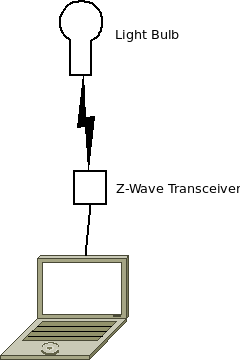
\includegraphics[width=0.75\columnwidth]{figs/testbedexp.png}                 
    \caption{Testbed Setup}                                                       
    \label{Fig:testsetup}                                                             
\end{figure} 
Our current testbed consists of a computer running Ubuntu 14.04, a Z-Wave
transceiver USB dongle, a Zipato RGBW Light Bulb. Figure~\ref{Fig:testsetup}
provides an overview of the testbed setup. Figure .. shows the test application
running.

Our system running on the laptop uses MySQL for the data backend. We are using
a command line interface to interact with the core sytem. We have a driver
running for the Z-Wave protocol and the Zipato RGBW Light Bulb. We also
developed an application, which when run, turns on the light bulb for two
seconds and then turns it off. 

When we run the application, the application goes to the Management Component
and requests the module for the ``Light Bulb'' role. The Managmenet Component
responds with a reference to the drivers for the Zipato RGBW Light Bulb. The
application then tells the driver to turn on the light bulb for two seconds and
then turn it off. The code snippet of the application can be viewed in the
Figure~\ref{Fig:appcode}.

